
\documentclass[fleqn,addpoints]{exam}
\usepackage{amsmath}
\usepackage{graphicx}
\usepackage{booktabs}
\usepackage{float}
\usepackage{caption}
\usepackage{polynom}
\usepackage{mdwlist}
\usepackage{cancel}

\usepackage{unitsdef} 
\newunit{\inch}{in}
\newunit{\mile}{mile}
\newunit{\mph}{mph}
\newunit{\foot}{ft}
\newunit{\knot}{knot}
\newunit{\gallon}{gallon}

\bracketedpoints
\everymath{\displaystyle}

\printanswers

\ifprintanswers 
\usepackage{2in1, lscape} 
\fi


% \begin{figure}[H]
%   \centering
%   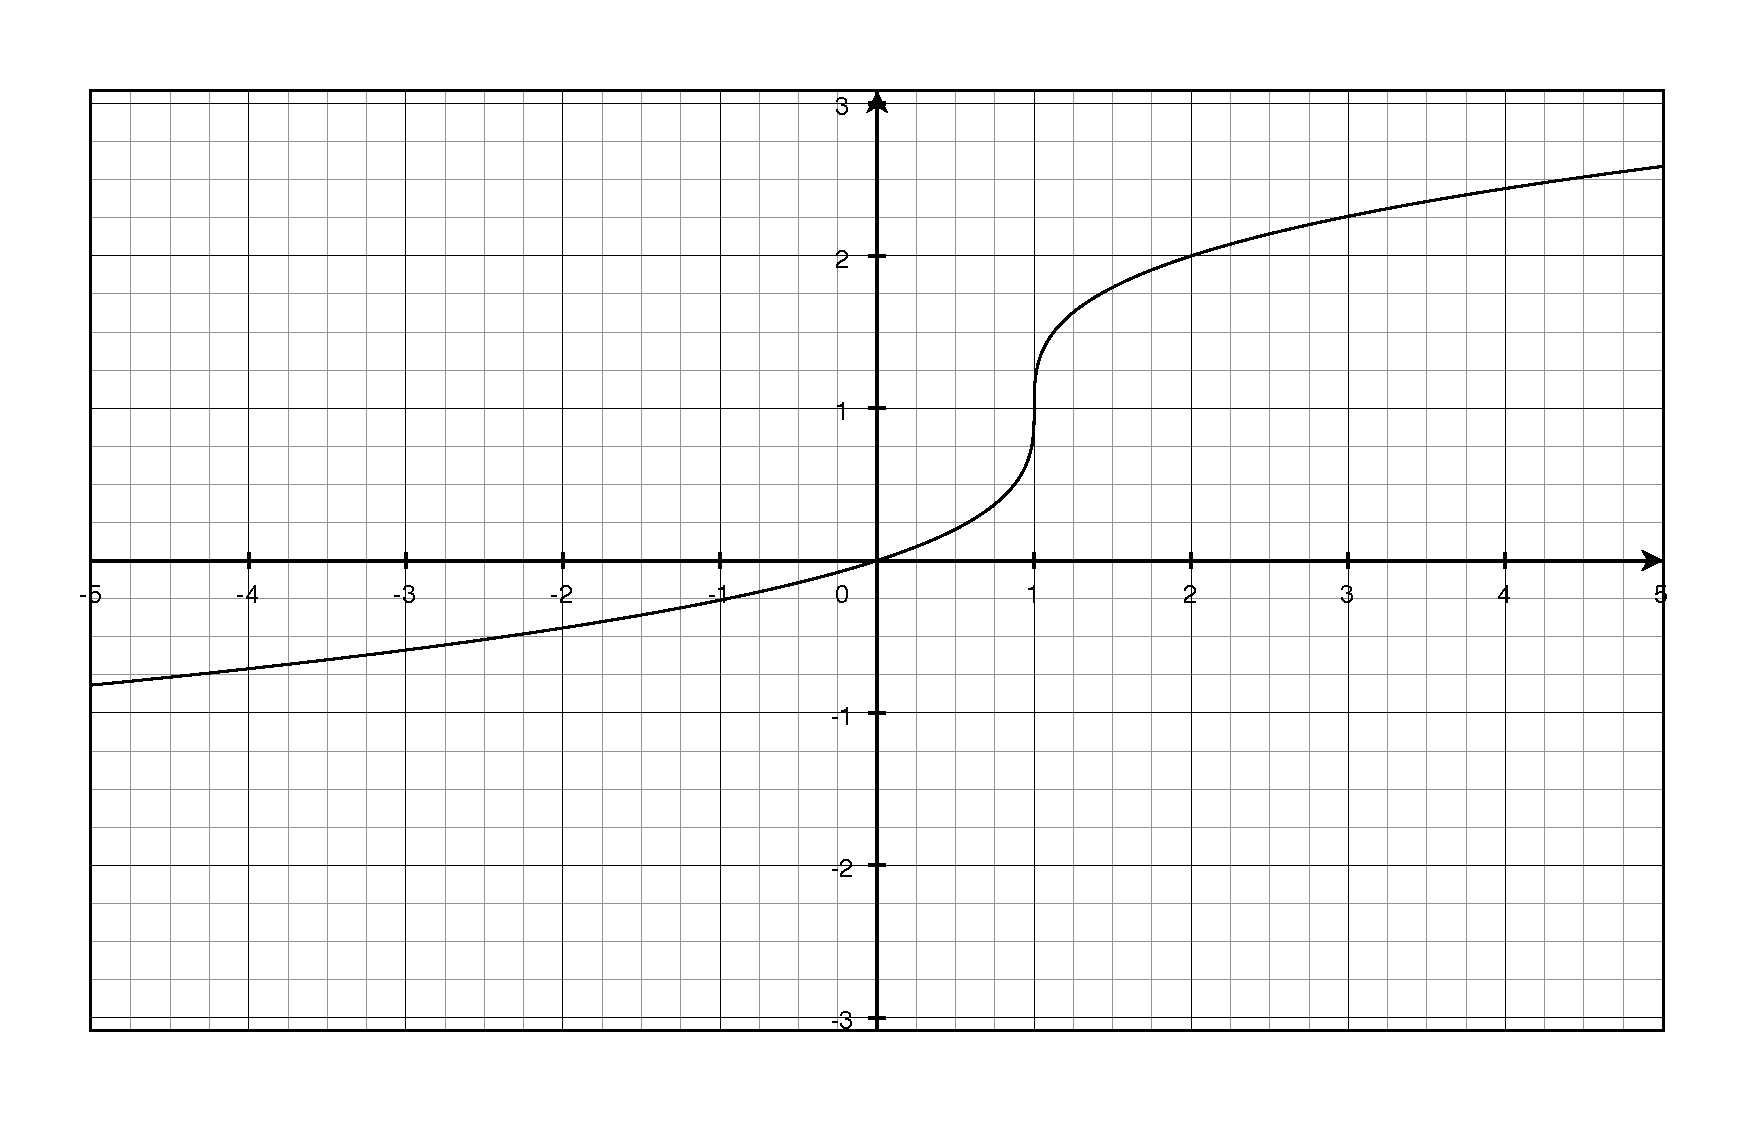
\includegraphics[scale=.3]{question7.eps}
%   \caption*{Question 7}
% \end{figure}

% \begin{tabular}{cc}
% \toprule
% period & amplitude \\
% \midrule
%   $\pi$ & $2$ \\
% \bottomrule
% \end{tabular}


%% \ifprintanswers
%% \usepackage{2in1, lscape}
%% \fi

\title{Math 263A Final Practice Problems One}
\date{October 18, 2012}

\author{}

\begin{document}

\maketitle  

\begin{questions}

\question Sketch the graph of a function that has a removable discontinuity at $x = 2$, a jump
discontinuity at $x = 4$ and a vertical asymptote at $x = 0$.

\begin{solution}
I can't get my computer to draw these graphs.
\end{solution}

\question
Use differentials to approximate $\sqrt[3]{8.02}$.

\begin{solution}
\begin{align*}
  f(x) &= x^{1/3} \\
  dy &= \frac{1}{3} x^{-2/3} \, dx \\
     &= \frac{0.02}{12} \\
     &= \frac{1}{600} \\
     &= 0.001667 \\
\\
  \sqrt[3]{8.02} &= 2.001667 \\
\end{align*}

\end{solution}

\ifprintanswers
\pagebreak
\fi

\question
$y = 2 \tan x \sin y$.  Find $\frac{dy}{dx}$ by implicit differentiation.
\begin{solution}
\begin{align*}
  y &= 2 \tan x \sin y \\
  y' &= 2 ( \tan x \cdot \cos y \cdot y' + \sin y \sec^2 x) \\
  y' - 2 y' \tan x \cos y &= \sin y \sec^2 x \\
  y' &=  \frac{\sin y \sec^2 x}{1 - 2 \tan x \cos y} \\
\end{align*}

\end{solution}

\question
$g(t)= \sqrt{t-1}$.  Find $g'$ using the definition of derivative. State the domain
of $g$ and the domain of $g'$.

\begin{solution}

\begin{align*}
  g'(t) &= \lim_{h \to 0} \frac{\sqrt{t - 1 + h} - \sqrt{t - 1}}{h} \\
  &= \lim_{h \to 0} \frac{t - 1 + h - (t - 1)}{h \left( \sqrt{t - 1 + h} + \sqrt{t - 1} \right)} \\
  &= \lim_{h \to 0} \frac{\cancel{h}}{\cancel{h} \left( \sqrt{t - 1 + h} + \sqrt{t - 1} \right)} \\
  &= \lim_{h \to 0} \frac{1}{\sqrt{t - 1 + h} + \sqrt{t - 1}} \\
  &= \frac{1}{2 \sqrt{t - 1}} \\
\end{align*}

The domain of $g$ is $[1, \infty)$ and the domain of $g'$ is $(1, \infty)$

\end{solution}

\ifprintanswers
\pagebreak
\fi

\question
$y = \sec \left( \frac{1}{x} \right)$.  Find $y'$.

\begin{solution}

If you don't have the derivative of $\sec x$ memorized, you can figure it out first:
\begin{align*}
  D_x \sec x &= D_x ( \cos x )^{-1} \\
  &= - (\cos x)^{-2} \cdot (- \sin x) \\
  &= \frac{\sin x}{\cos^2 x} \\
  &= \tan x \sec x \\
\end{align*}

Now you're ready to solve the original problem:
\begin{align*}
  D_x \sec ( x^{-1} ) &= \tan (x^{-1}) \sec (x^{-1}) \cdot (-x^{-2}) \\
  &= - \frac{\tan (1/x) \sec(1/x)}{x^2} \\
\end{align*}

\end{solution}

\question $f(x)= \frac{2x}{x+1}$.  Find an equation of the tangent line to the curve at $(1, 1)$.

\begin{solution}
First you need to find the value of the derivative at that point, so that you'll have the slope:
\begin{align*}
  f'(x) &= \frac{(x + 1) \cdot 2 - 2x}{(x + 1)^2} \\
  &= \frac{2}{(x + 1)^2} \\
\\
  f'(x) &= \frac{1}{2} \\
\end{align*}

So the equation of the line is: 
\begin{align*}
  y - 1 &= \frac{1}{2}(x - 1) \\
  y &= \frac{1}{2} x + \frac{1}{2} \\
\end{align*}

\end{solution}

\question A man starts walking north at 4 ft/s from a point P. Five minutes later a woman starts walking south at 5 ft/s
from a point 500 ft due east of P. At what rate are the people moving apart 15 min after the woman starts walking.

\begin{solution}
One thing to watch out for in this one is that the rates are in seconds but the times are in minutes.  It's easiest to
convert everything to seconds. 

It's also easiest to make $t = 0$ be the time when the woman starts walking.

At time zero, the man has been walking for 300 seconds, so he is already 1,200 feet away.  The equation
for the man's y-position is: $y_m = 1200 + 4t$.

Since the woman is at the origin at time zero, the equation her y-position is: $y_w = 5t$.

Since the two people are moving in opposite directions, the total $y$ position is: $y_{total} = 1200 + 9t$.

Neither person is moving in the $x$ direction.

The distance between the two people is: $r^2 = x^2 + y^2$.  We're looking for $\frac{dr}{dt}$, which we can find with
implicit differentiation:

\begin{align*}
  r^2 &= x^2 + y^2 \\
  2r \frac{dr}{dt} &= 2x \frac{dx}{dt} + 2y \frac{dy}{dt} \\
  \frac{dr}{dt} &= \frac{x}{r} \frac{dx}{dt} + \frac{y}{r} \frac{dy}{dt}
\end{align*}

This is the same equation you get for all these types of problems.  You should also memorize this equation and go back and check your work
if you end up with something different.

To get the actual value for $\frac{dr}{dt}$, plug in all the numbers we have.  The time is 900 seconds after the start.
\begin{itemize}
  \item $y(900) = 9300$
  \item $x(900) = 500$
  \item $r(900) \approx 9313$
  \item $\frac{dy}{dt} = 9$
  \item $\frac{dx}{dt} = 0$
\end{itemize}

\begin{align*}
  \frac{dr}{dt} &= \frac{9300}{9313} \cdot 9 \\
  &\approx 8.99 \ \foot/\second \\
\end{align*}

\end{solution}

\question Find the dimensions of the rectangle of largest area that can be inscribed in an equilateral triangle of side
$L$ if one side of the rectangle lies on the base of the triangle.

\begin{solution}
Before you start this one, you should draw a picture of the rectangle inscribed in the triangle.  I placed the triangle
so the origin is at the midpoint of the bottom side of the triangle.
 
For problems where you're inscribing something in something else, you need to use the outer figure to get an equation
for the line which must contain the point which maximizes the area of the inner figure.

If $L$ is the length of a side, the height of the triangle is:
\begin{align*}
  \left( \frac{L}{2} \right)^2 + h^2 &= L^2 \\
  h &= \frac{\sqrt{3}}{2} L \\
\end{align*}
Now we can find the equation for the line on the right side of the triangle.  The y-intercept is the height, and the
slope is:
\[
  m = - \frac{\left( \cfrac{\sqrt{3}}{2} L \right)}{\left( \cfrac{L}{2} \right) } = - \sqrt{3} 
\]
So the equation for the line on the right side of the triangle is: $y = - \sqrt{3} x + \frac{\sqrt{3}}{2} L$

The area of the rectangle is the base times the height:
\begin{align*}
  A &= 2x \cdot \left( - \sqrt{3} x + \frac{\sqrt{3}}{2} L \right) \\
    &= - 2 \sqrt{3} x^2 + \sqrt{3} xL \\
\end{align*}

To find the maximum area, we need to take the derivative and set it equal to zero:
\begin{align*}
  A' &= -4 \sqrt{3} x + \sqrt{3} L \\
\\
  0 &= -4 \sqrt{3} x + \sqrt{3} L \\
  4 \sqrt{3} x &= \sqrt{3} L \\
  x &= \frac{L}{4} \\ 
\end{align*}

\end{solution}

\question Evaluate: $\lim_{x \to \infty} \frac{2x^3 + 10 x^2 - 7x}{4x^3 +2x^2 + 3}$

\begin{solution}
Since the degree of the numerator is equal to the degree of the denominator, you can just glance at the equation and see
that the limit is $\frac{1}{2}$.  

For a test, however, you should show a little work:
\[
  \lim_{x \to \infty} \frac{2x^3 + 10 x^2 - 7x}{4x^3 +2x^2 + 3} 
      = \lim_{x \to \infty} \frac{2 + 10/x - 7/x^2}{4 +2/x + 3/x^2} 
  = \frac{2}{4} 
  = \frac{1}{2}
\]

\end{solution}

\question $f(x) = x^4 - 6x^2$

\begin{parts}
\part Find the vertical and horizontal asymptotes.

\begin{solution}
  Since this isn't a rational function, there aren't any asymptotes.
\end{solution}

\part Find the intervals on which f is increasing or decreasing.

\begin{solution}
To do this we need to use the first derivative test.
\begin{align*}
  f'(x) &= 4x^3 - 12x \\
  4x^3 - 12x &= 0 \\
  x(x^2 - 3) &= 0 \\
  x &= \{-\sqrt{3}, 0, \sqrt{3}\} \\
\end{align*}

If you try a few test points or do a sign chart, you can see that $f$ is 
\begin{itemize*}
  \item increasing on $\left(- \sqrt{3}, 0 \right) \cup \left( \sqrt{3}, \infty \right)$  
  \item decreasing on $\left( -\infty, -\sqrt{3} \right) \cup \left( 0, \sqrt{3} \right)$  
\end{itemize*}

Notice that you don't include the endpoints in any of these intervals.  The derivative at the endpoint is 0, so the
function isn't increasing or decreasing there.

\end{solution}

\part Find the local maximum and minimum values of $f$.
\begin{solution}
From the previous step, we can see that the local maximum occurs at $x = 0$ and the local minimums occur at 
$x = \pm \sqrt{3}$. 

\begin{itemize*}
  \item The maximum is $(0, 0)$
  \item The minimums are $\left( \pm \sqrt{3}, -9 \right)$
\end{itemize*}

\end{solution}

\ifprintanswers
\pagebreak
\fi

\part Find the intervals of concavity and the inflection points.

\begin{solution}
Use the second derivative test:
\begin{align*}
  f'(x) &= 12x^2 - 12 \\
\\
  12x^2 - 12 &= 0 \\
  x &= \pm 1 \\
\end{align*}

The graph is concave up from $\left(-\infty, -1 \right] \cup \left[1, \infty \right)$ and concave down from $[-1, 1]$.  The
  inflection points are $(\pm 1, -5)$.

\end{solution}

\part Use the information from (a)-(d) to sketch the graph.
\begin{solution}
\begin{figure}[H]
  \centering
  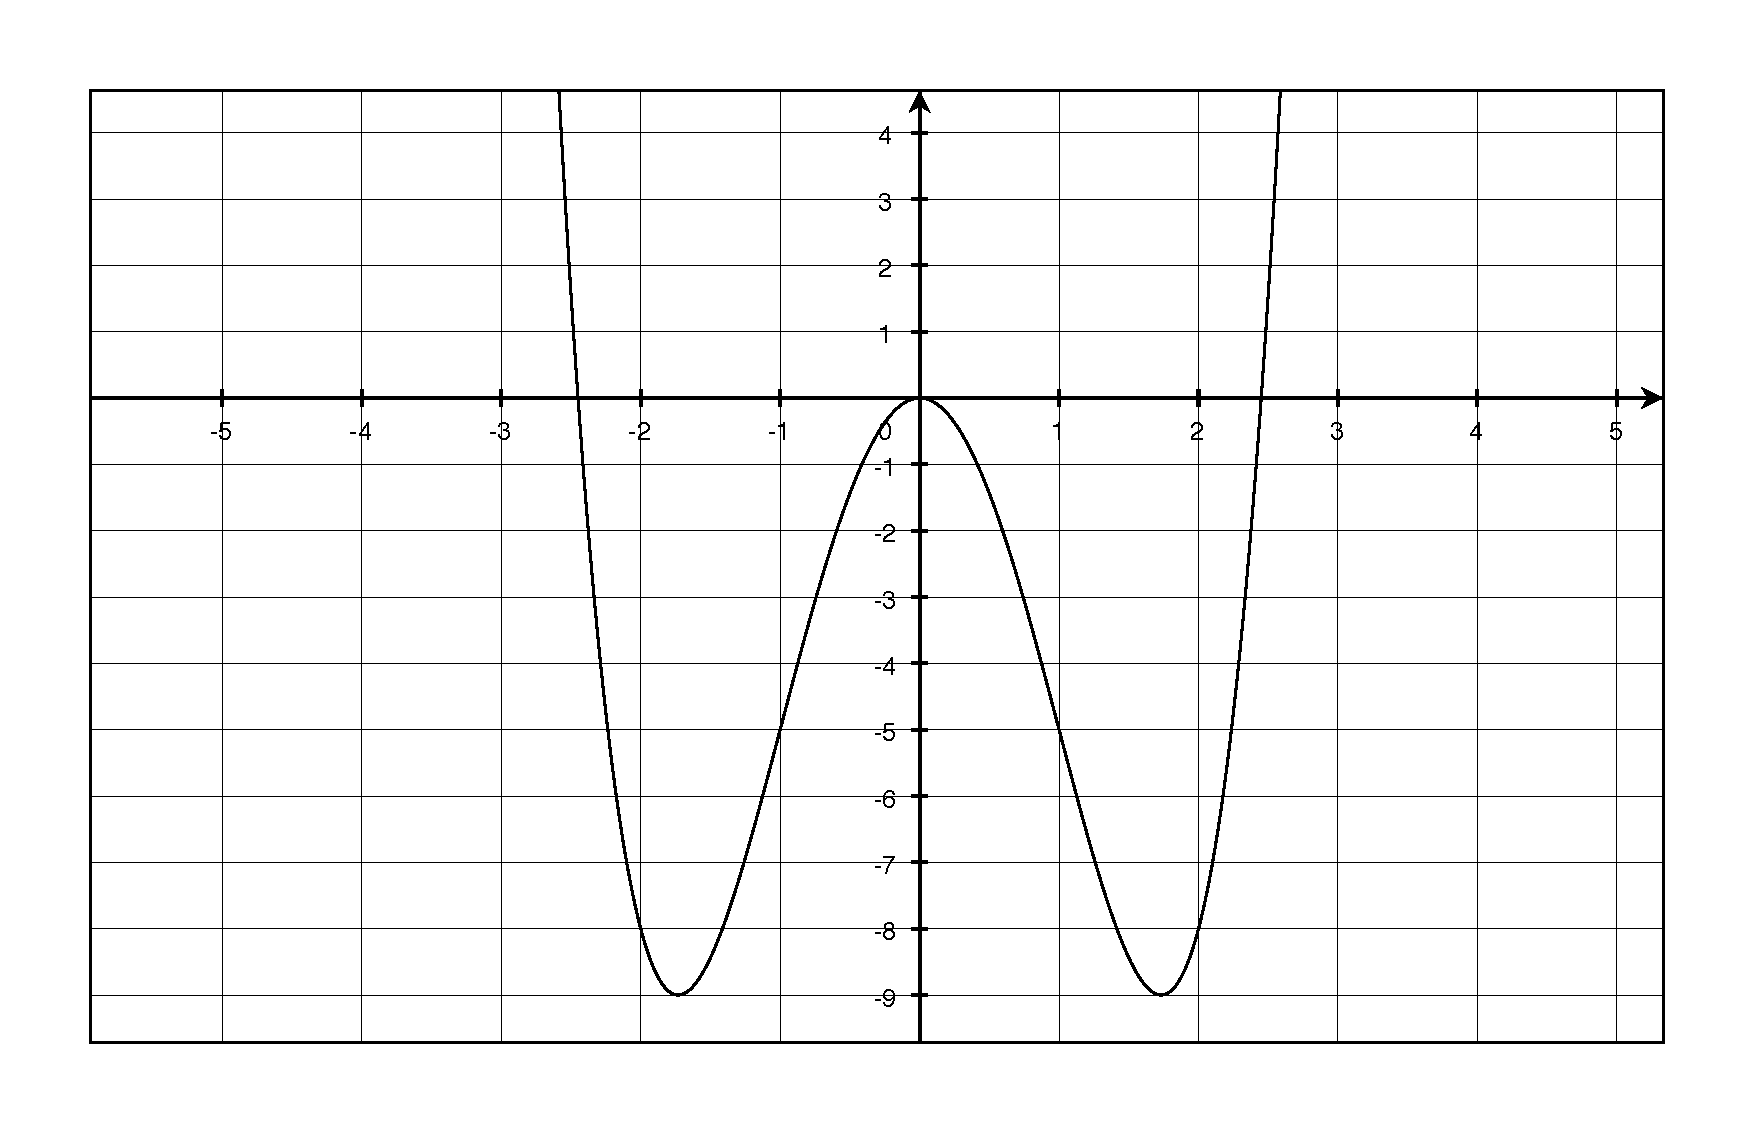
\includegraphics[scale=.3]{practice_q10.eps}
  \caption*{Question 10}
\end{figure}
\end{solution}

\end{parts}

\end{questions}

\end{document}
